\documentclass{beamer}
\usepackage{default}
\usepackage{pgfpages}
\usepackage{tikz}
\usepackage{mathtools}
\renewcommand{\thefootnote}{}
\usepackage{colortbl}
\usepackage{hyperref}
\usepackage{multimedia}
\title{Git Review}
\begin{document}


\begin{frame}
\begin{center}
 \texttt{Git}: Branching and Merging
 \vspace{30pt}
 
 Molly Gibson\\
 @gibsmk
\end{center}
\end{frame}

\begin{frame}
\frametitle{What is a branch?}
A branch is just a pointer to a commit:
\begin{center}
\scalebox{0.7}{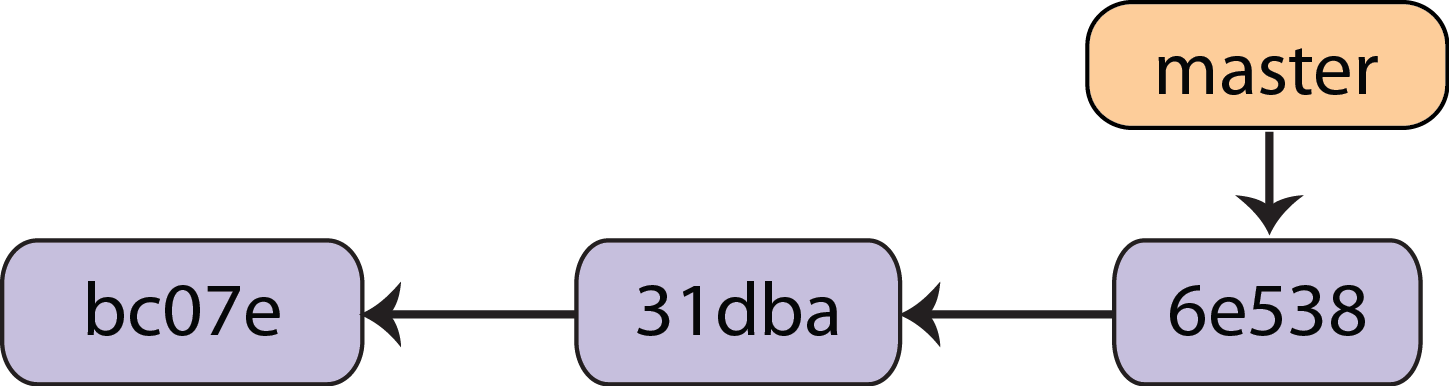
\includegraphics{../imgs/branch1.png}}

\vspace{20pt}
We have been using the \texttt{master} branch.
\end{center}

\end{frame}

\begin{frame}[fragile]
\frametitle{Intro to Branching}
We can create a new branch and it will add a new pointer to the current commit:
\begin{center}
\scalebox{0.7}{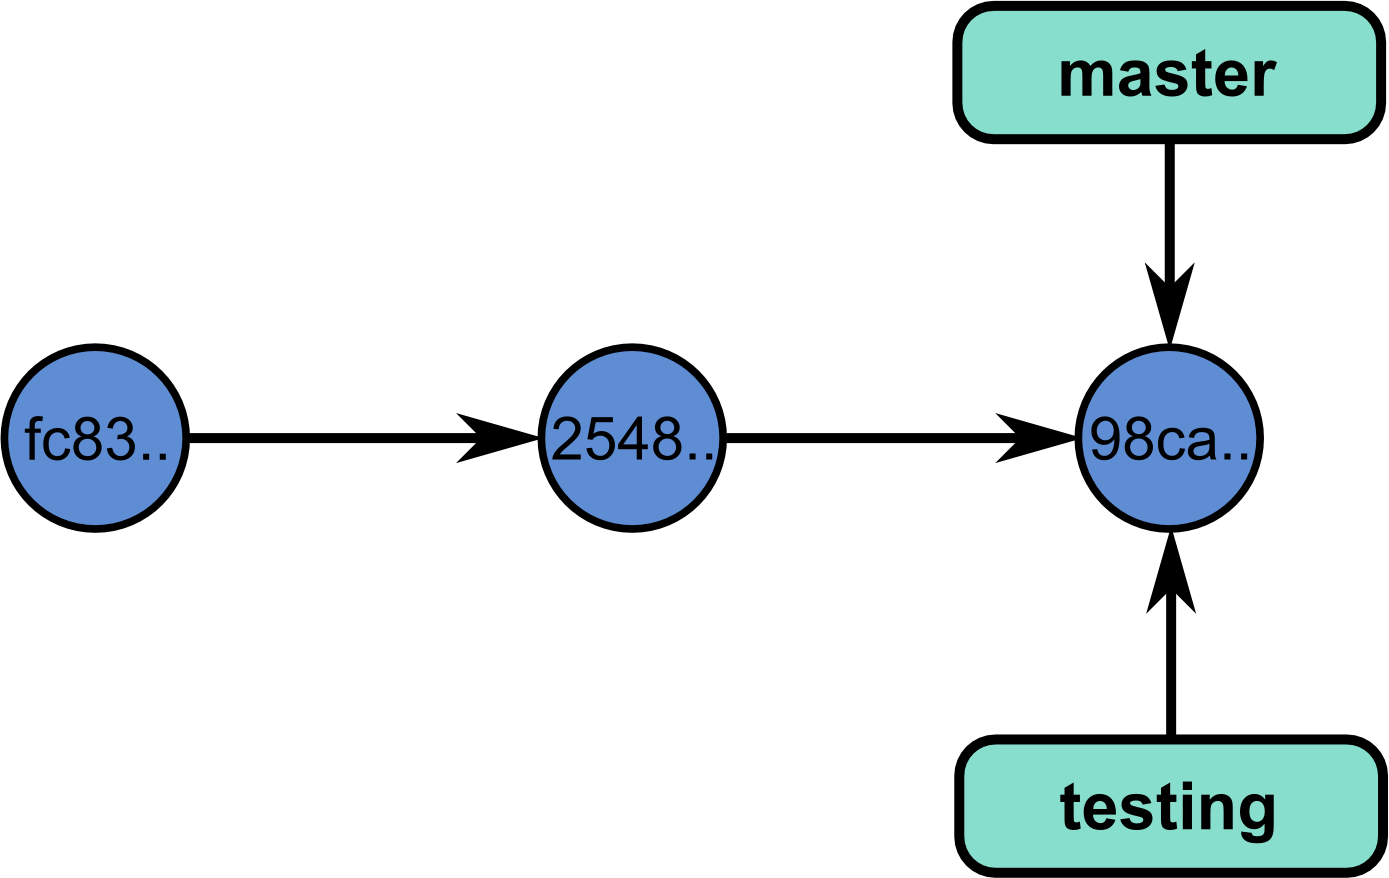
\includegraphics{../imgs/branch2.png}}

\begin{verbatim}
                   git branch test
\end{verbatim}
\end{center}
\end{frame}

\begin{frame}
\frametitle{Intro to Branching}
How does \texttt{Git} know which branch you are currently on? 
\begin{center}
\scalebox{0.6}{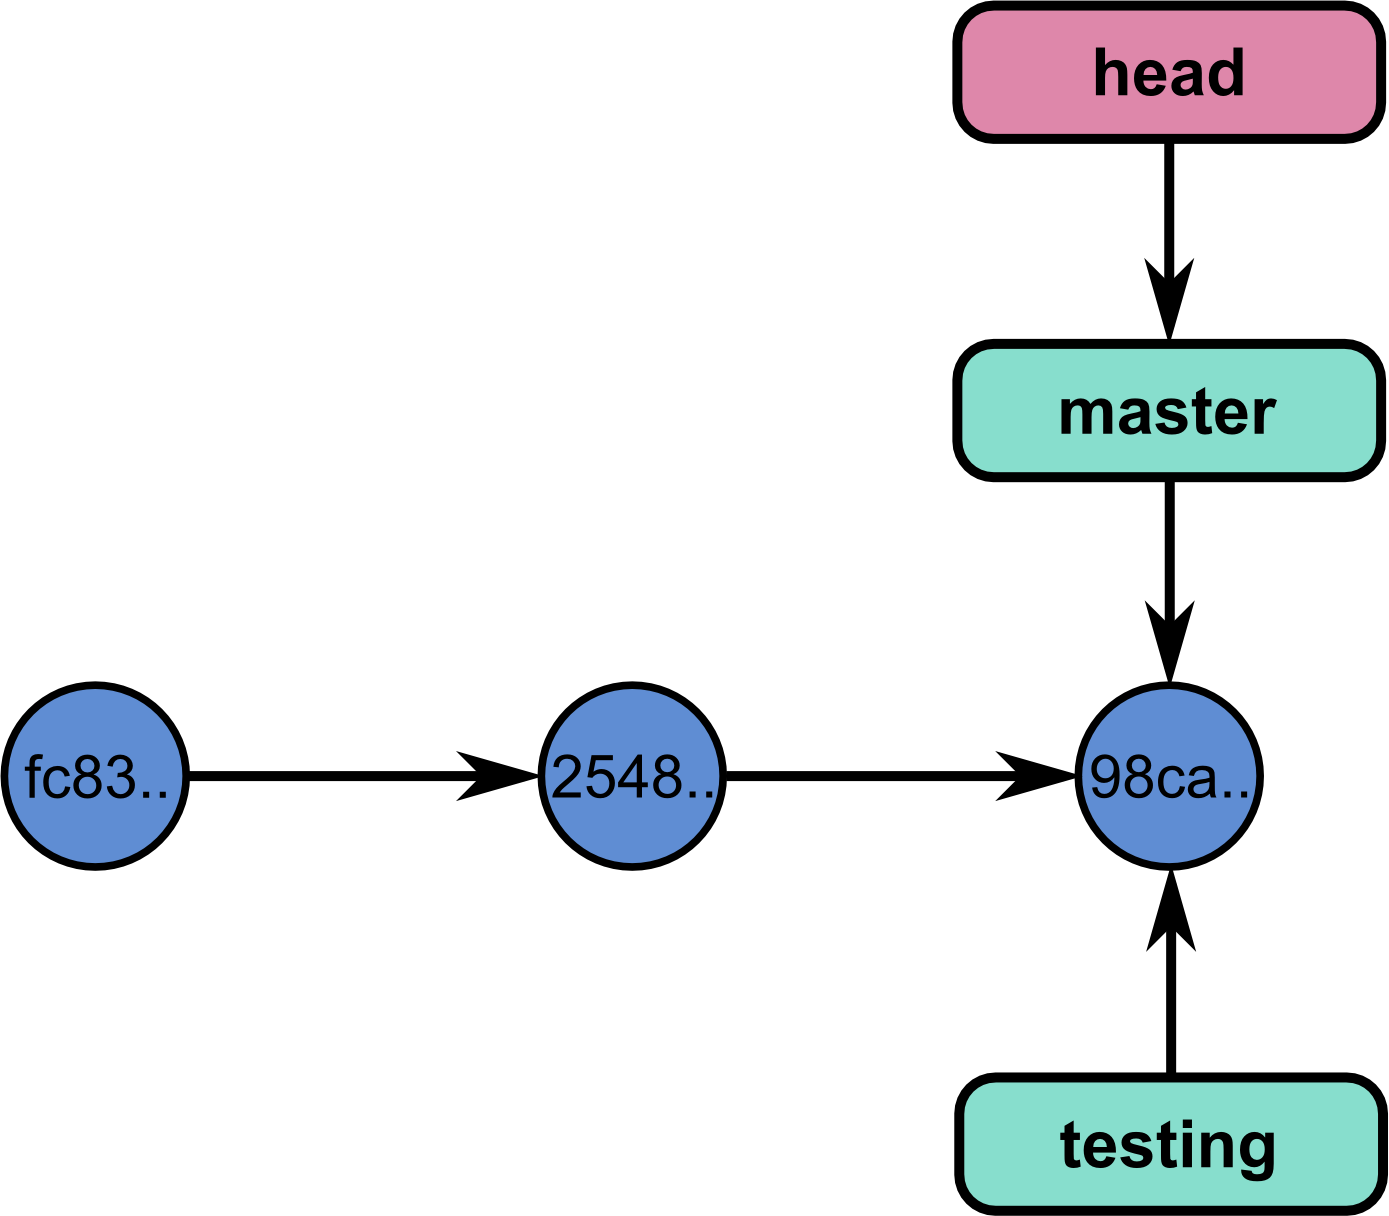
\includegraphics{../imgs/branch3.png}}

\end{center}
\end{frame}

\begin{frame}[fragile]
\frametitle{Intro to Branching}
You can change the current branch by using \texttt{git checkout}:
\begin{center}
\scalebox{0.6}{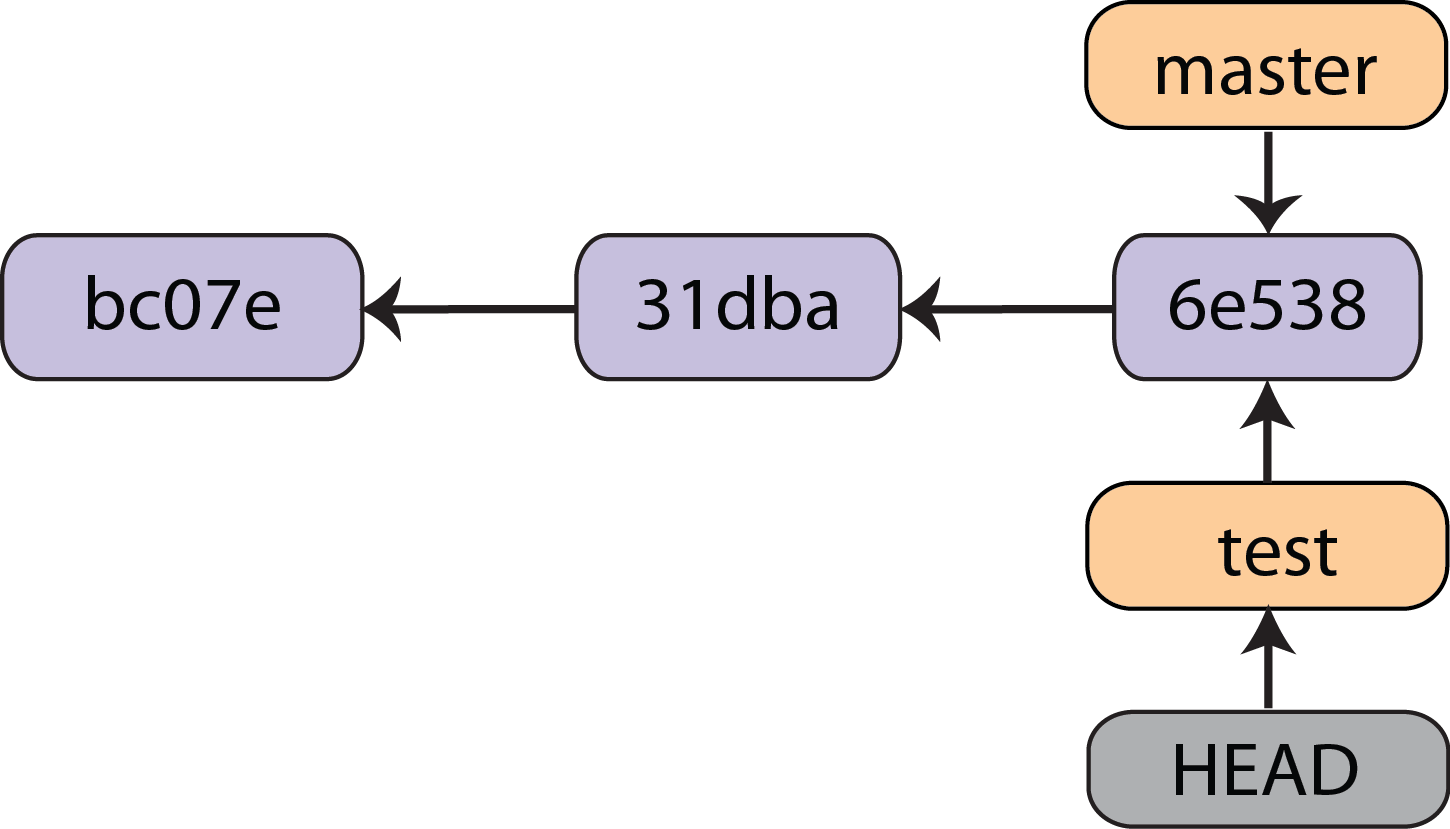
\includegraphics{../imgs/branch3-5.png}}

\begin{verbatim}
                   git checkout test
\end{verbatim}
\end{center}

\end{frame}


\begin{frame}
\frametitle{Intro to Branching}
If you add commits on both branches, the directories can diverge:
\begin{center}
\scalebox{0.5}{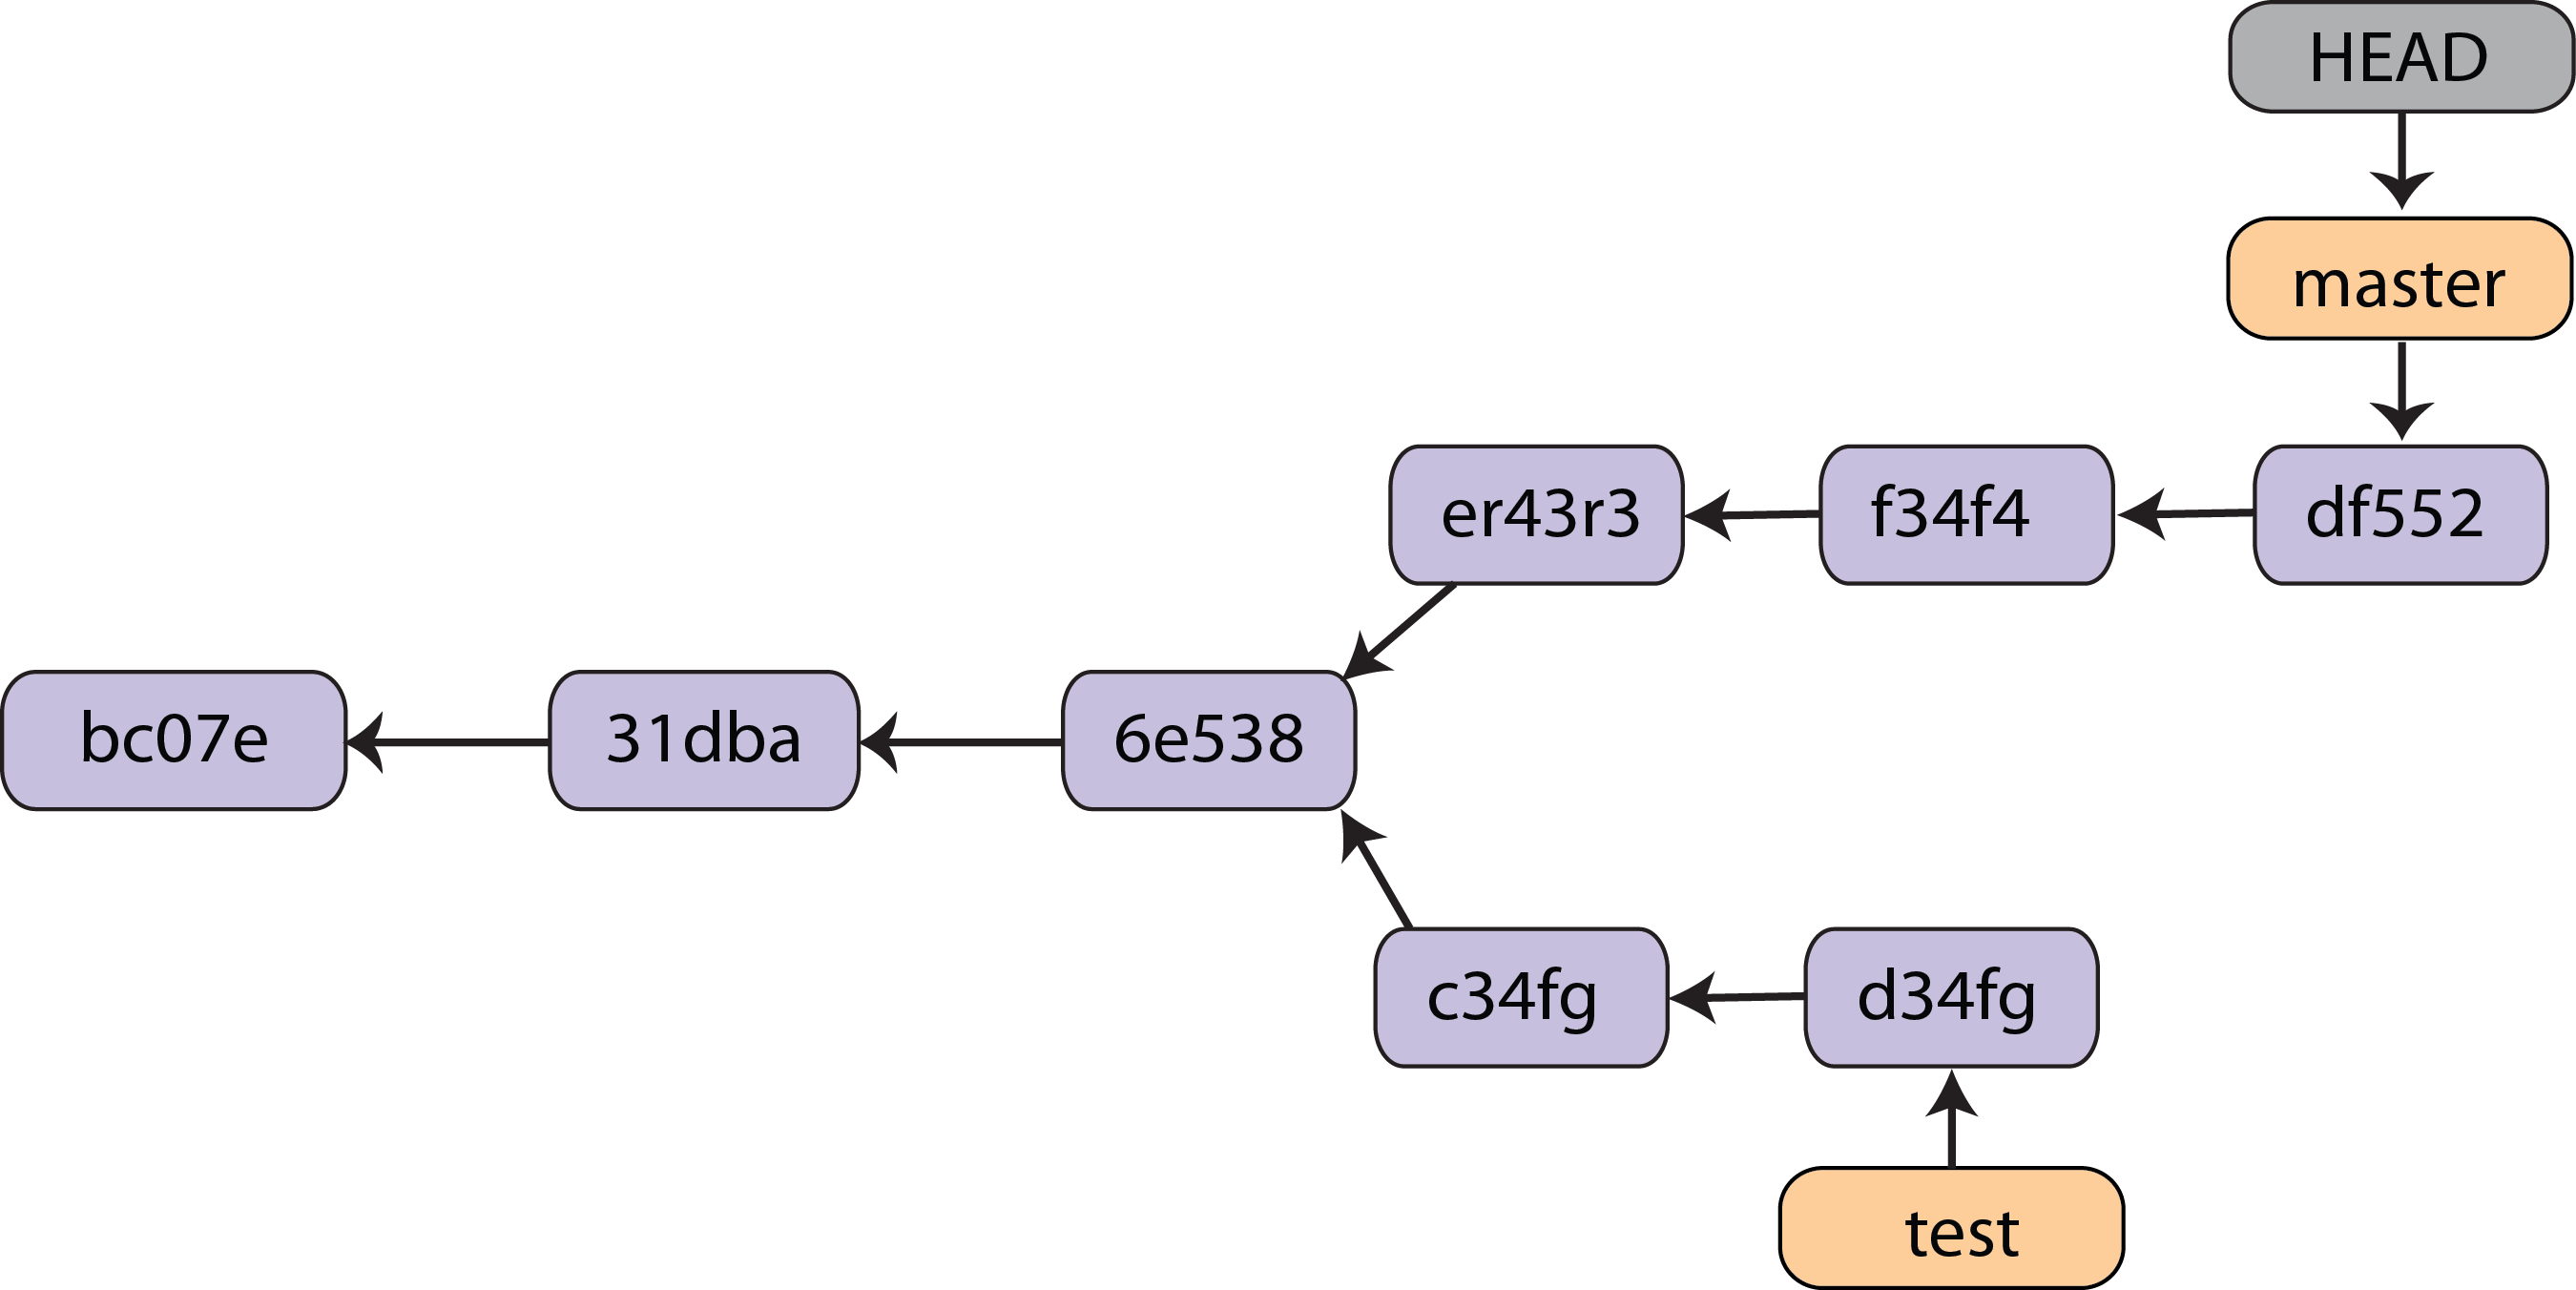
\includegraphics{../imgs/branch4.png}}

\end{center}
\end{frame}

\begin{frame}[fragile]
\frametitle{Intro to Branching}
Eventually, you might want to merge your changes on your branch back into the master development branch:
\begin{center}
\scalebox{0.45}{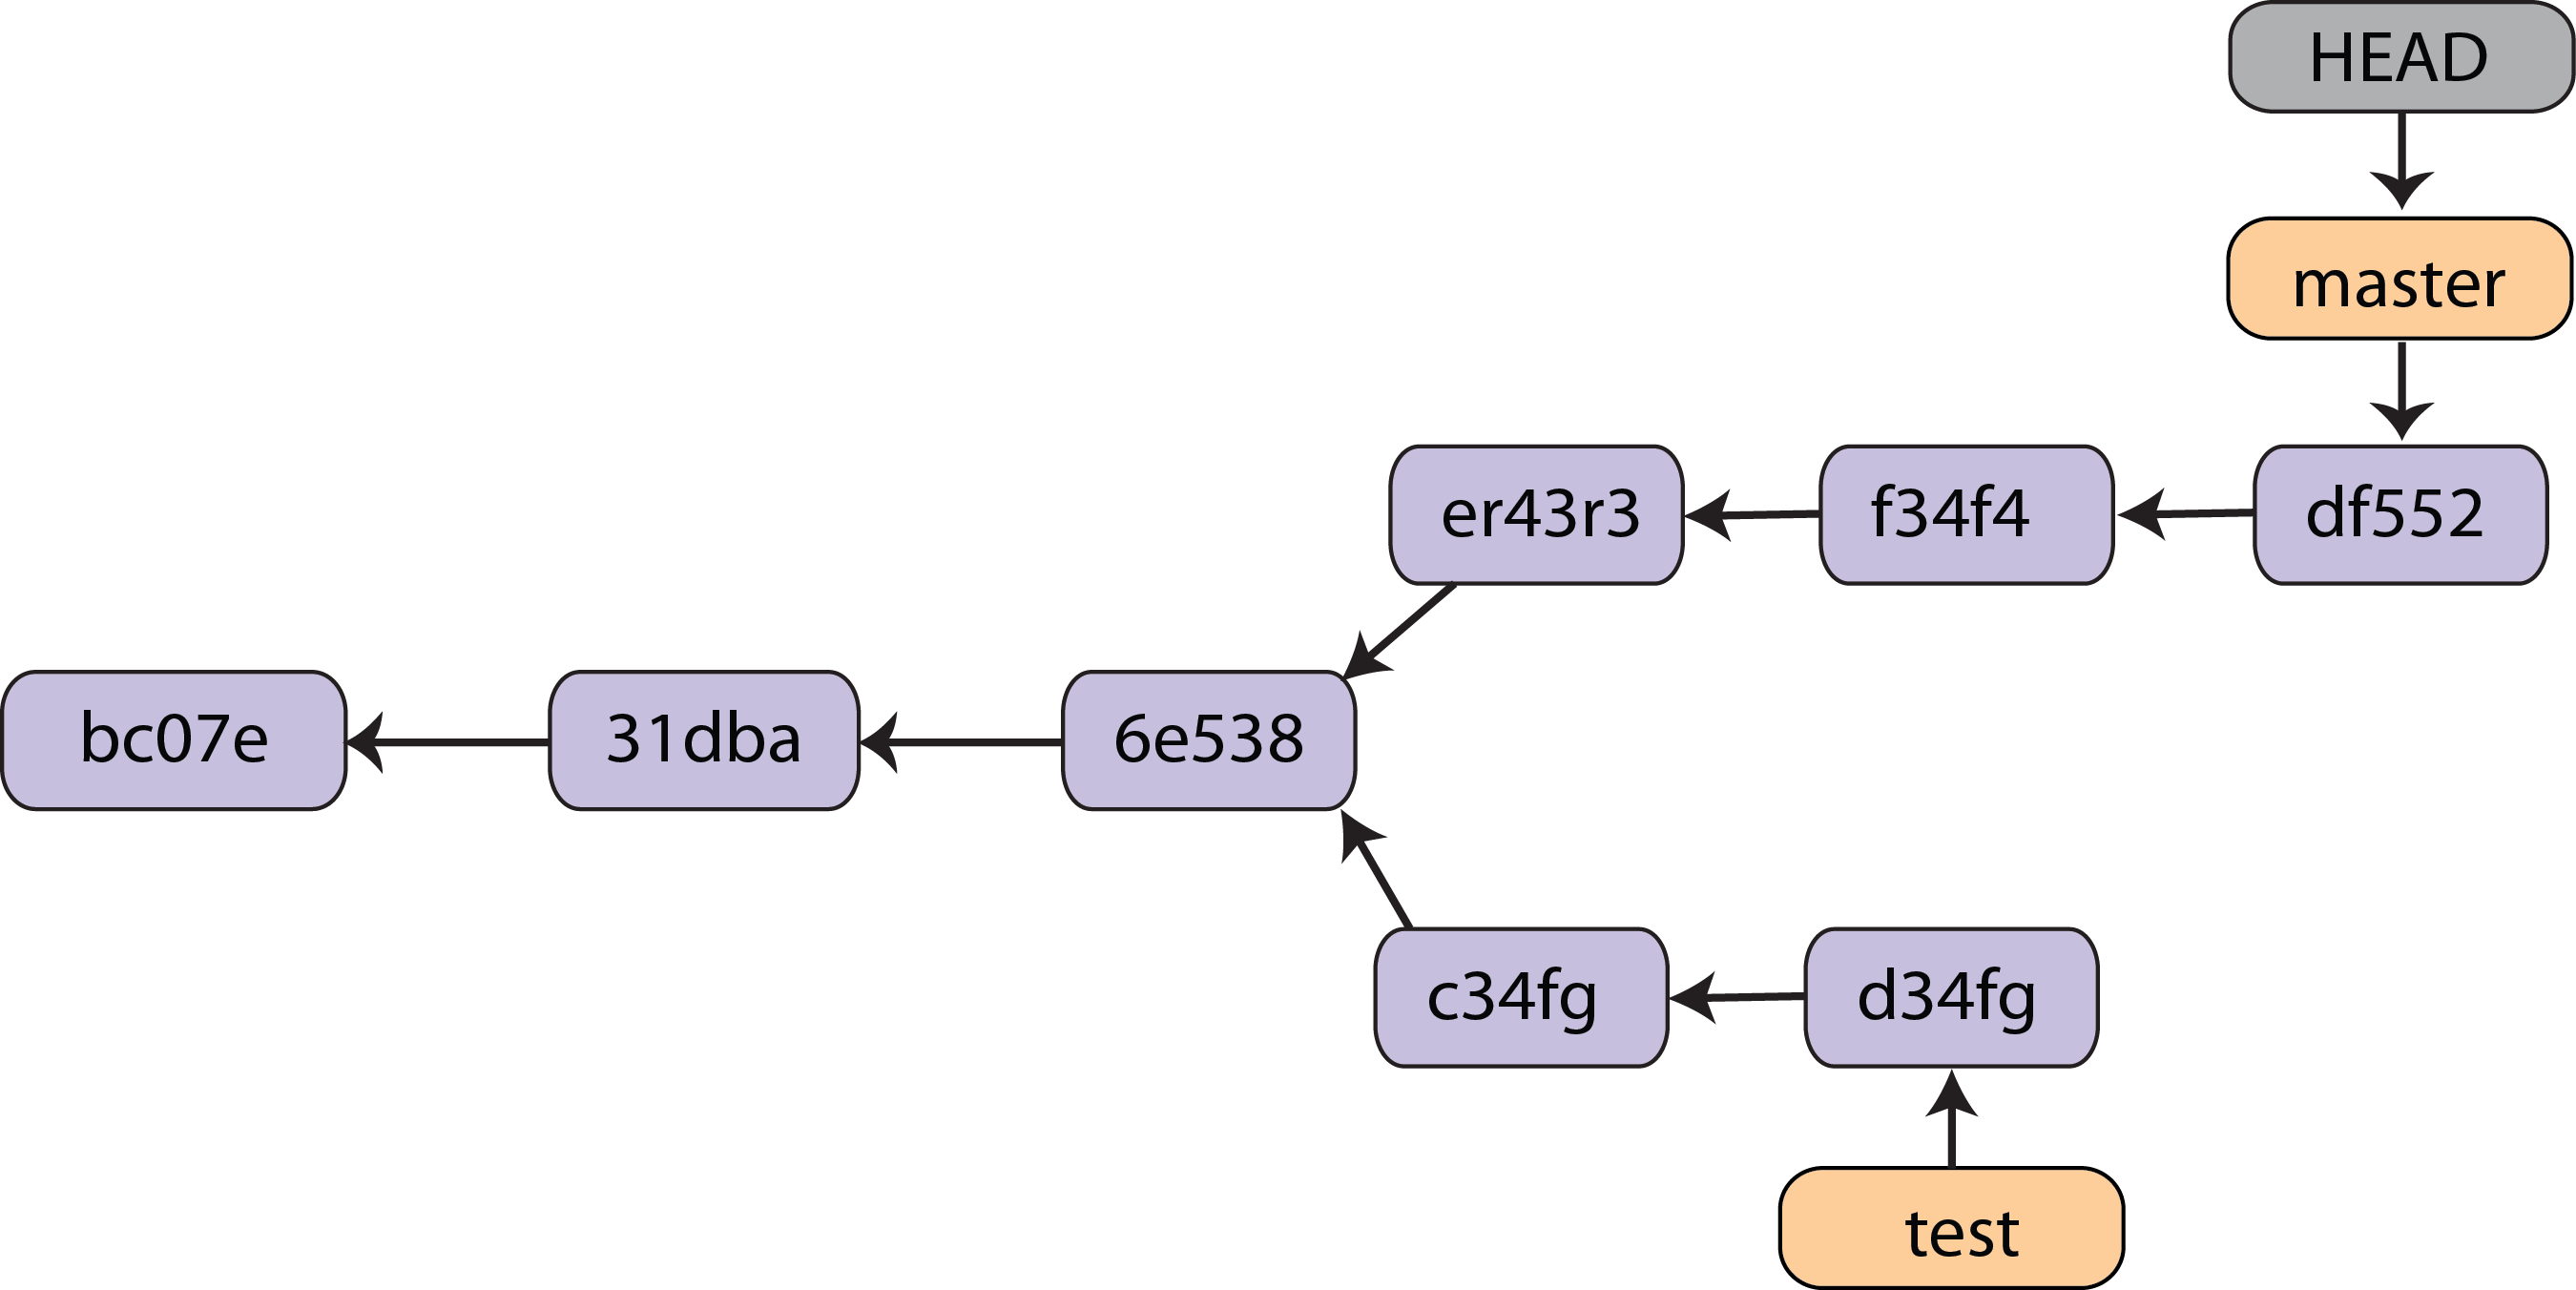
\includegraphics{../imgs/branch5.png}}
\begin{verbatim}
                   git merge test
\end{verbatim}
\end{center}
\end{frame}

\begin{frame}[fragile]
\frametitle{Resolving Conflicts}
Inevitably, you will get this error at some point when merging:
\begin{verbatim}
$ git merge test
Auto-merged file1.txt
CONFLICT (content): Merge conflict in file1.txt
Automatic merge failed; fix conflicts and then 
commit the result.
\end{verbatim}
\end{frame}

\begin{frame}[fragile]
\frametitle{Resolving Conflicts}
This has now been put in the conflicting file:
\begin{verbatim}
<<<<<<< HEAD:file1.txt
This is in the master branch.
=======
This is in the test branch.
>>>>>>> test:file1.txt
\end{verbatim}\pause
\textit{Let's see how you resolve a merge conflict.}
\end{frame}


\begin{frame}
\frametitle{Why branch?}
\begin{center}
Isolation of changes. \pause
\vspace{15pt}

Try new things without disrupting main code. 
\end{center} \pause

Usually, there are a few main types of branches:
\begin{enumerate}
\item Feature Branch
\begin{itemize}
\item If a particular feature is disruptive enough that you don't want the entire development team to be affected in its early stages, you can create a branch on which to do this work.
\end{itemize}
\item Fixes Branch
\begin{itemize}
\item While development continues on the main trunk, a fixes branch can be created to hold the fixes to the latest released version of the software.
\end{itemize}
\end{enumerate} 
\end{frame}


\begin{frame}
\frametitle{Your Turn}
\begin{center}
Questions? \pause
\vspace{30pt}

You Try (30 mins) \\\
\textbf{\textcolor{red}{Exercise 5}}
\end{center}
\end{frame}


\end{document}


